\subsection{Messungen von AnkleRoll zum Test}

Die Messungen von LAnkleRoll und RAnkleRoll, zu sehen in Abb. \ref{hardware_llegjoint} und \ref{hardware_rlegjoint} wurden 20 mal wiederholt und mit den normalen Schuhen von Nao vollzogen. Dabei legte er in etwa eine Strecke von $0,8 \unit{m}$ auf der Rampe im flachen Zustand zurück. Insgesamt wurden alle verfügbaren Messwerte von AnkleRoll aufgezeichnet, das sind pro Aktor 6 Messwerte. Temperatur, Stiffness und Temperatur Status erwiesen sich als Konstant und daher nicht entscheidend, um einen Unterschied der Bodenbeschaffenheit oder Sohlen erkennen zu können. Stiffness ist immer auf $100\%$ während dem Gang. 
Der Befehl für diesen Lauf war der moveTo() Befehl, welcher nicht weiter verändert wurde (kommt in den Theorieteil).


In Abb. \ref{AnkleRoll_links_act} und \ref{AnkleRoll_rechts_act} sind die Messdaten von jeweils einem Fuß des Messwertes Position/Actuator abgebildet. Hier ist zu sehen, dass die Anfangswerte sich aufspalten, in positive und einmal in negative Winkelangaben. Dies ist der Tatsache geschuldet, dass die Funktion moveTo() per Zufall Nao mit dem linken oder mit dem rechten Fuß beginnen lässt. 

Dies wurde für Abb. \ref{AnkleRoll_beide_act_sens_links_anfang} und \ref{AnkleRoll_beide_act_sens_rechts_anfang} sortiert. In ersterer Abbildung beginnt Nao mit dem linken Fuß. Da die Hüfte sich für den ersten Schritt nach rechts bewegen muss, verschiebt sich die Position beider Gelenke in die Negativrichtung, der Winkel wird absolut gemessen, wie in Abb \ref{hardware_llegjoint} und \ref{hardware_rlegjoint} zu sehen ist. 

Außerdem sind in Abb. \ref{AnkleRoll_beide_act_sens_links_anfang} und \ref{AnkleRoll_beide_act_sens_rechts_anfang} neben den Messwerten von Position Actuator in schwarz auch die von Position Sensor in blau gezeigt. \textcolor{red}{Was diese beiden Messwerte genau unterscheidet und ob einer von moveTo() vorgegeben wird, ist noch zu entscheiden.} Der bedeutenste Unterschied ist zu Beginn der Aufnahmen. Die Position/Actuator Messung beginnt nahe 0, während Position/Sensor für den jeweiligen Fuß bei einem Wert über Null oder unter Null anfängt. 

Es ist eindeutig zu erkennen, dass die Messungen erst nach der Sortierung des Anfangsschrittes ein regelmäßiges Bild ergeben. 

Der Strom, welcher die Gelenke einsetzen müssen um das gewollte Ergebnis zu erzielen, scheint eine mögliche, vergleichbare Aufnahmegröße für unterschiedliche Sohlen und Umgebungen des Nao zu sein. In Abb. \ref{AnkleRoll_beide_current_links_anfang} und \ref{AnkleRoll_beide_act_sens_rechts_anfang} ist der Messwert Current aufgeteilt in Anfangsschritte gezeigt. Hier ist der Unterschied, mit welchem Fuß der erste Schritt gemacht wird, nicht so gravierend, wie bei den vorherigen Messwerten. Allerdings zeichnet sich eine Tendenz ab, dass der linke Fuß, hier in schwarz, einen höheren Strom beansprucht, als der rechte Fuß. Dies könnte dem beobachteten Fehlgang des Naos und dem zusätzlichen Geräusch bei jedem zweiten Schritt geschultet sein. Bei normaler Einstellung und ohne Korrektur würde dieser Nao einen Bogen nach rechts laufen. Um dies auszugleichen wurden bei moveTo() Anpassungen hinzugefügt.   

\begin{figure}[tb]
	\centering
	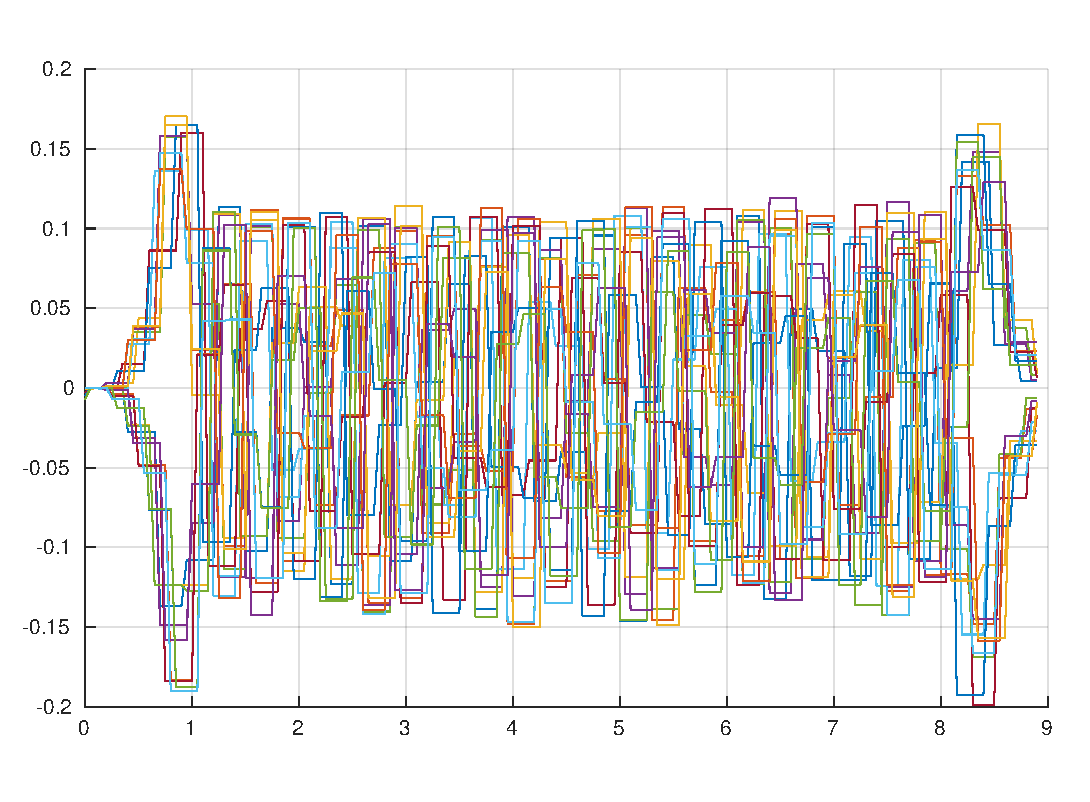
\includegraphics[width=1\linewidth]{Bilder/AnkleRoll_links_act.pdf}
	\caption{AnkleRoll Messwert Position Actuator des linken Fußes}
	\label{AnkleRoll_links_act}
\end{figure}

\begin{figure}[tb]
	\centering
	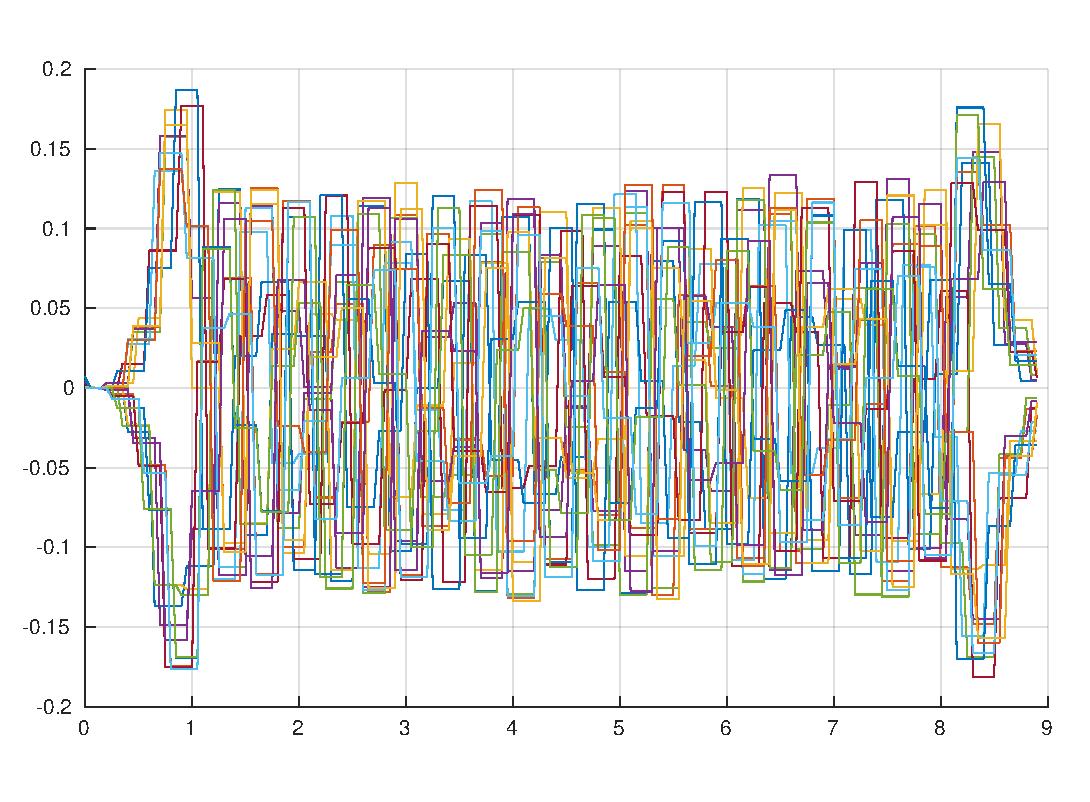
\includegraphics[width=1\linewidth]{Bilder/AnkleRoll_rechts_act.pdf}
	\caption{AnkleRoll Messwert Position Actuator des rechten Fußes}
	\label{AnkleRoll_rechts_act}
\end{figure}
\begin{figure}[tb]
	\centering
	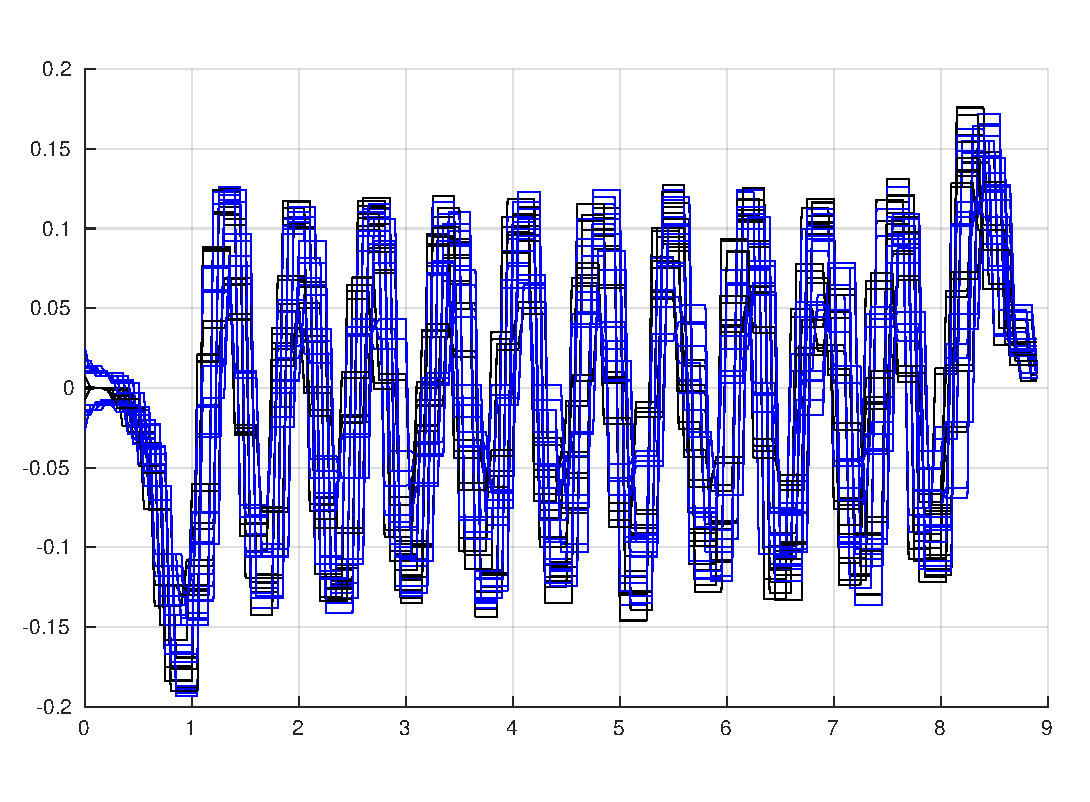
\includegraphics[width=1\linewidth]{Bilder/AnkleRoll_beide_act_sens_links_anfang.pdf}
	\caption{AnkleRoll Aktoren beider Seiten mit dem Position/Actuator Messwert in schwarz und dem Position/Sensor Messwert in blau. Nao macht hier den ersten Schritt mit Links.}
	\label{AnkleRoll_beide_act_sens_links_anfang}
\end{figure}
\begin{figure}[tb]
	\centering
	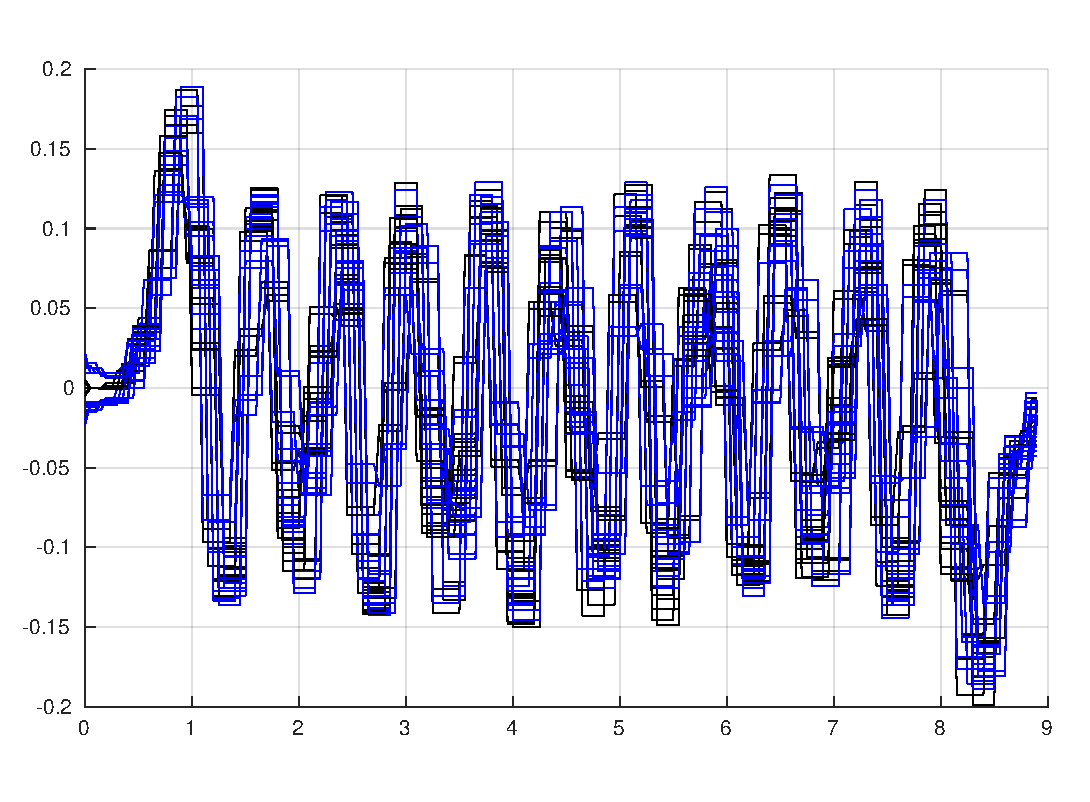
\includegraphics[width=1\linewidth]{Bilder/AnkleRoll_beide_act_sens_rechts_anfang.pdf}
	\caption{AnkleRoll Aktoren beider Seiten mit dem Position/Actuator Messwert in schwarz und dem Position/Sensor Messwert in blau. Nao macht hier den ersten Schritt mit Rechts.}
	\label{AnkleRoll_beide_act_sens_rechts_anfang}
\end{figure}
\begin{figure}[tb]
	\centering
	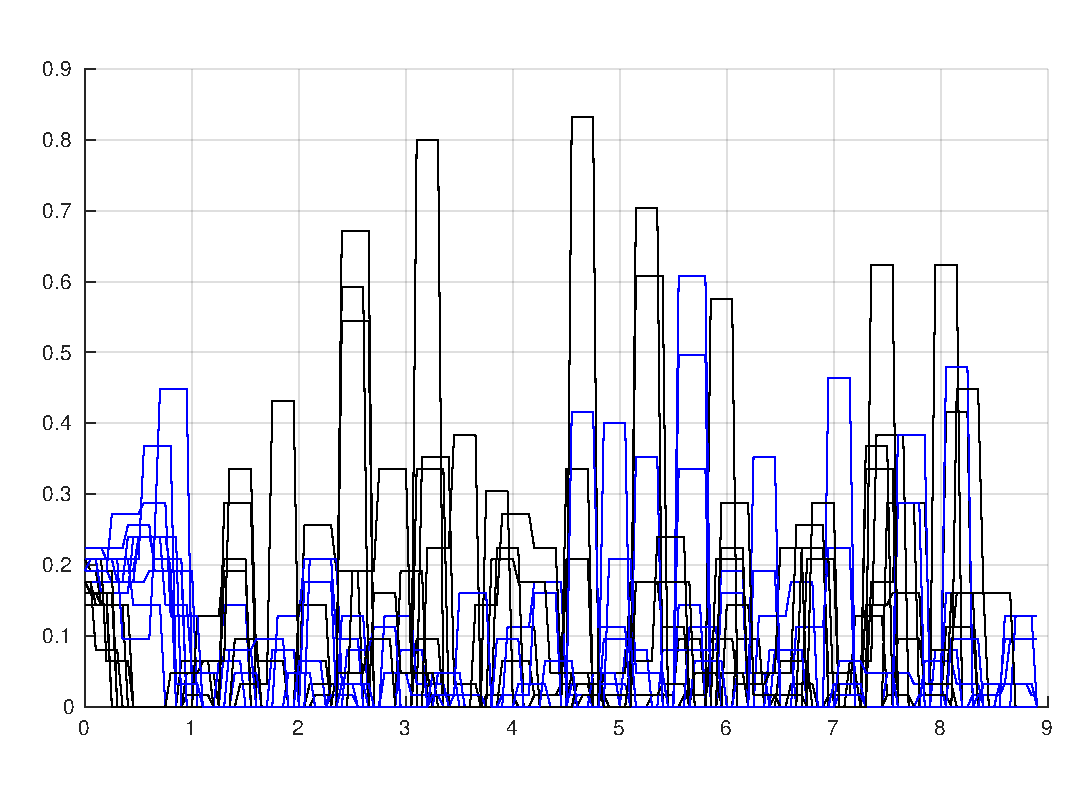
\includegraphics[width=1\linewidth]{Bilder/AnkleRoll_beide_current_links_anfang.pdf}
	\caption{AnkleRoll Aktoren beider Seiten mit dem Current Messwert. Messwert Links ist in Schwarz, Messwert Rechts ist in Blau. Nao macht hier den ersten Schritt mit Links.}
	\label{AnkleRoll_beide_current_links_anfang}
\end{figure}
\begin{figure}[tb]
	\centering
	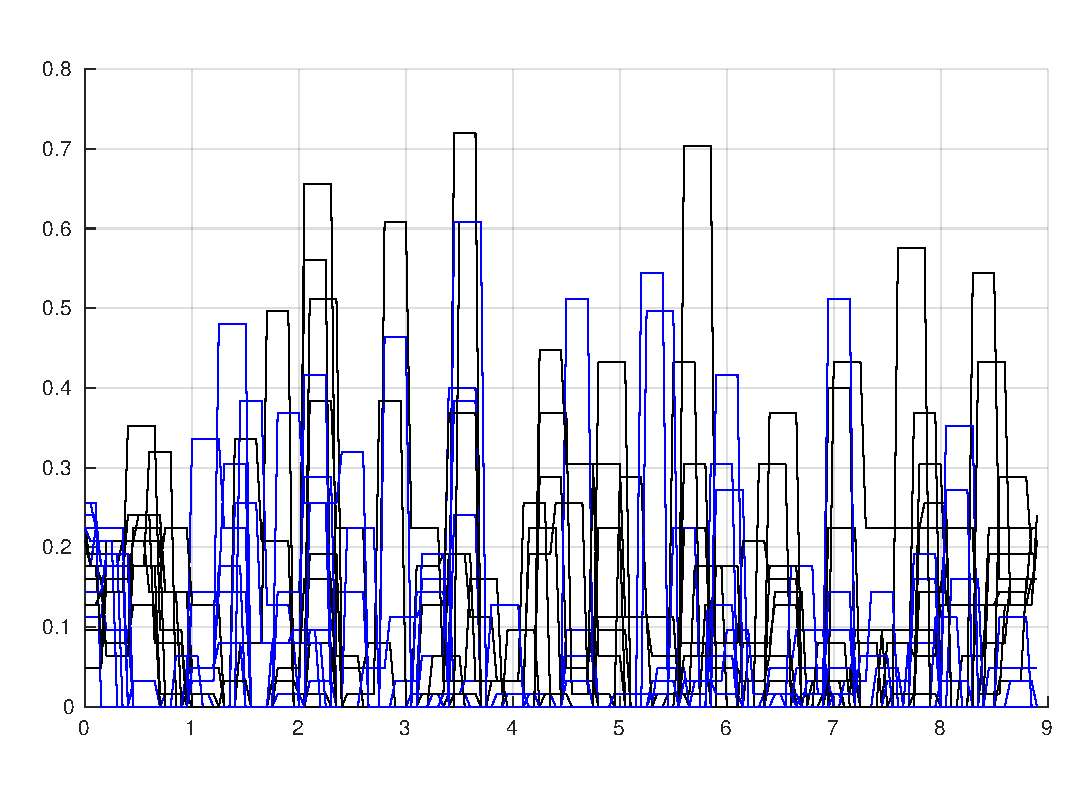
\includegraphics[width=1\linewidth]{Bilder/AnkleRoll_beide_current_rechts_anfang.pdf}
	\caption{AnkleRoll Aktoren beider Seiten mit dem Current Messwert. Messwert Links ist in Schwarz, Messwert Rechts ist in Blau. Nao macht hier den ersten Schritt mit Rechts.}
	\label{AnkleRoll_beide_current_rechts_anfang}
\end{figure}
%%% Local Variables:
%%% mode: latex
%%% TeX-master: "main"
%%% End: